%\graphicspath{ {./sea_vs_blue_f781c5/} }
\graphicspath{ {../figures/} }

\chapter{Seastore OSD: single vs. dual Seastar reactor per core}

In this Chapter we show the comparison of Seastore (build 6aab5c07ae) on longer
duration test sets, producing response latency curves. 

The single reactor per CPU core configuration is shown in Figure
\ref{figure:sea_1osd_single_reactor_conf}, whereas the dual reactor
configuration is shown in Figure \ref{figure:sea_1osd_dual_reactor_conf}.
In both cases, we use the balanced OSD method.

\begin{figure}[!ht]
  \centering
  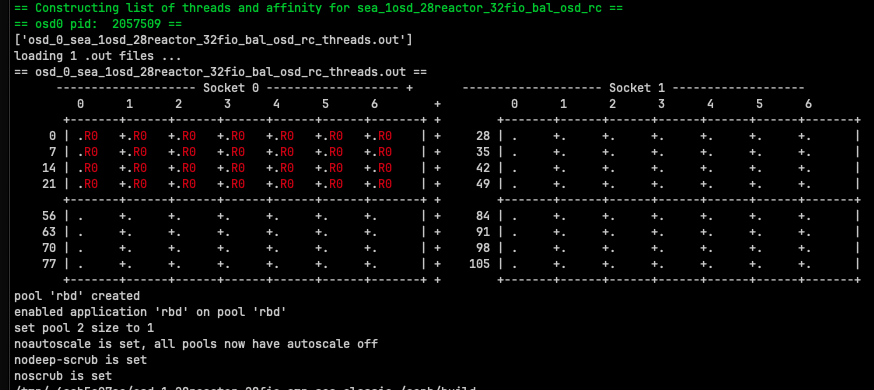
\includegraphics[width=0.9\textwidth]{sea_1osd_single_reactor_conf.png}
  \caption{Single reactor per physical CPU core configuration.}
  \label{figure:sea_1osd_single_reactor_conf}
\end{figure}


\begin{figure}[!ht]
  \centering
  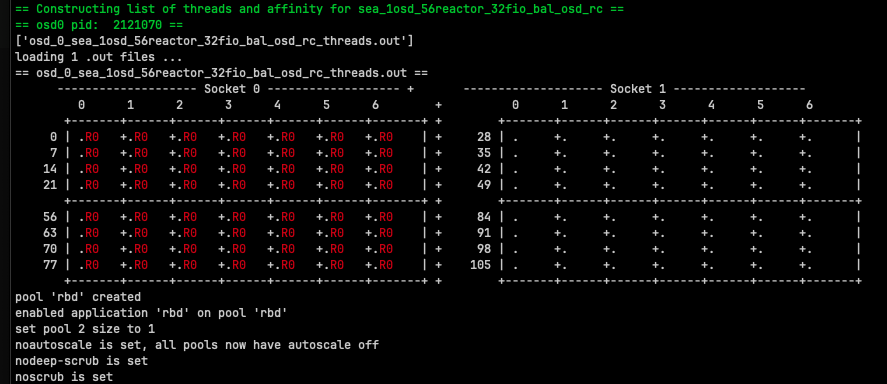
\includegraphics[width=0.9\textwidth]{sea_1osd_dual_reactor_conf.png}
  \caption{Dual reactor per physical CPU core configuration.}
  \label{figure:sea_1osd_dual_reactor_conf}
\end{figure}


% The curves show the standard deviation of the mean of the
% latency as vertical error bars, the smaller the bar, the better (less
% variation). 
Unfortunately, there seemed to have occurred several failures, since the OSD
pid being monitored does not appear the whole duration of the test in the
performance data. This is reflected in zero valued OSD measurements. The test
drive script does not expected the pid for the process OSD to change for the
lifetime of the cluster. Consequently this also affects the benchmark data, as
shown by the considerable fluctuations.

Despite this, the results below show that the dual configuration achieves
better performance than the single reactor configuration. 
\pagebreak
\section{Random read 4k}

\begin{figure}[!ht]
  \centering
  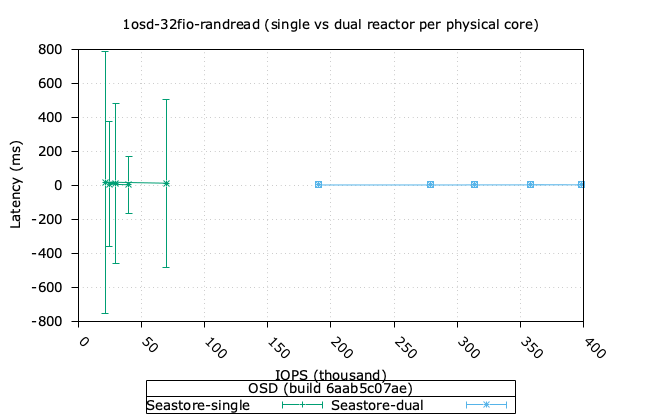
\includegraphics[width=0.9\textwidth]{seastore_1osd_32fio_randread_iops_vs_lat.png}
  \caption{Response latency curves, IOPs vs. Latency}
\end{figure}

% utilisation:OSD
% \begin{figure}[h]
%   \centering
%   \begin{minipage}{.5\textwidth}
%   \centering
%     \includegraphics[width=\textwidth]{classic_vs_seastore_1osd_32fio_randread_iops_vs_lat_osd_cpu.png}
%     %\caption{4k random read}
%      %\label{figure:sea_4k_randread}
%   \end{minipage}%
%   \begin{minipage}{.5\textwidth}
%   \centering
%     \includegraphics[width=\textwidth]{classic_vs_seastore_1osd_32fio_randread_iops_vs_lat_osd_mem.png}
%     %\caption{System CPU utilisation}
%     %\label{figure:sea_4k_randwrite}
%   \end{minipage}%
% \end{figure}
%
%In the Tables below we show the performance figures for the workloads above.
% Table showing the figures for this workload
\subsection{Single reactor}
../data//osd_1_28reactor_28fio_rc_seastore/sea_1osd_28reactor_32fio_bal_osd_rc_1procs_randread_d/sea_1osd_28reactor_32fio_bal_osd_rc_1procs_randread.tex
\subsection{Dual reactor}

\begin{table}[h!]
\centering
\begin{tabular}[t]{*{11 }{|c|}}
\hline 
iodepth & iops & total\_ios & clat\_ms & clat\_stdev & usr\_cpu & sys\_cpu & OSD\_cpu & OSD\_mem & FIO\_cpu & FIO\_mem\\
\hline
128  & 68695.43  & 4112383.00  & 0.40  & 62.70  & 1.06  & 1.00  & 1730.84  & 1961.00  & 290.20  & 0.00 \\
\hline

\hline
\end{tabular}
\caption{Performance Throughput vs Latency vs CPU util: sea_1osd_56reactor_32fio_bal_osd_rc_1procs_randread.}
\label{table:iops-lat-cpu-sea_1osd_56reactor_32fio_bal_osd_rc_1procs_randread}
\end{table}

%\newpage
\pagebreak

\section{Random write 4k}

\begin{figure}[ht!]
  \centering
  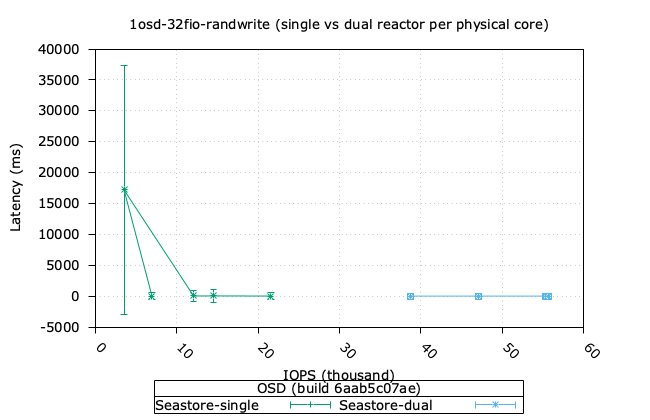
\includegraphics[width=0.9\textwidth]{seastore_1osd_32fio_randwrite_iops_vs_lat.png}
\end{figure}

% utilisation:OSD
% \begin{figure}[h]
%   \centering
%   \begin{minipage}{.5\textwidth}
%   \centering
%     \includegraphics[width=\textwidth]{classic_vs_seastore_1osd_32fio_randwrite_iops_vs_lat_osd_cpu.png}
%     %\caption{4k random write}
%      %\label{figure:sea_4k_randwrite}
%   \end{minipage}%
%   \begin{minipage}{.5\textwidth}
%   \centering
%     \includegraphics[width=\textwidth]{classic_vs_seastore_1osd_32fio_randwrite_iops_vs_lat_osd_mem.png}
%     %\caption{System CPU utilisation}
%     %\label{figure:sea_4k_randwrite}
%   \end{minipage}%
% \end{figure}
%
\subsection{Single reactor}

\begin{table}[h!]
\centering
\begin{tabular}[t]{*{11 }{|c|}}
\hline 
iodepth & iops & total\_ios & clat\_ms & clat\_stdev & usr\_cpu & sys\_cpu & OSD\_cpu & OSD\_mem & FIO\_cpu & FIO\_mem\\
\hline
1  & 462.66  & 20688.00  & 68.79  & 1718.76  & 0.01  & 0.01  & 0.00  & 0.00  & 2.35  & 9.00 \\
\hline
2  & 6974.29  & 347787.00  & 9.12  & 542.11  & 0.14  & 0.10  & 0.00  & 0.00  & 39.02  & 22.50 \\
\hline
4  & 3540.54  & 131.00  & 17200.65  & 20133.63  & 0.00  & 0.00  & 0.00  & 0.00  & 7.46  & 0.00 \\
\hline
8  & 12089.40  & 723780.00  & 21.07  & 838.38  & 0.23  & 0.16  & 0.00  & 0.00  & 66.76  & 29.49 \\
\hline
16  & 14523.08  & 1014684.00  & 34.72  & 1103.52  & 0.27  & 0.19  & 0.00  & 0.00  & 86.23  & 34.50 \\
\hline
24  & 21568.72  & 2369475.00  & 10.10  & 508.13  & 1.34  & 0.96  & 0.00  & 0.00  & 177.59  & 17.07 \\
\hline
32  & 8.41  & 419.00  & 35309.91  & 22885.21  & 0.00  & 0.00  & 0.00  & 0.00  & 7.28  & 0.85 \\
\hline
40  & 191.32  & 9529.00  & 5953.88  & 16170.11  & 0.01  & 0.00  & 0.00  & 0.00  & 9.61  & 1.50 \\
\hline
52  & 6594.02  & 1543.00  & 316.35  & 406.43  & 0.12  & 0.10  & 0.00  & 0.00  & 8.48  & 0.00 \\
\hline
64  & 6062.91  & 2795.00  & 436.46  & 599.57  & 0.14  & 0.13  & 0.00  & 0.00  & 10.15  & 1.50 \\
\hline

\hline
\end{tabular}
  \caption{Performance Throughput vs Latency vs CPU util: random write 4k, single reactor per CPU core.}
  %sea_1osd_28reactor_32fio_bal_osd_rc_1procs_randwrite.}
\label{table:iops-lat-cpu-sea_1osd_28reactor_32fio_bal_osd_rc_1procs_randwrite}
\end{table}

\subsection{Dual reactor}

\begin{table}[h!]
\centering
\begin{tabular}[t]{*{11 }{|c|}}
\hline 
iodepth & iops & total\_ios & clat\_ms & clat\_stdev & usr\_cpu & sys\_cpu & OSD\_cpu & OSD\_mem & FIO\_cpu & FIO\_mem\\
\hline
1  & 28788.24  & 8636588.00  & 1.11  & 0.91  & 0.65  & 0.48  & 0.00  & 0.00  & 220.87  & 52.50 \\
\hline
2  & 39690.09  & 11907224.00  & 1.61  & 1.63  & 0.77  & 0.58  & 0.00  & 0.00  & 273.56  & 79.50 \\
\hline
4  & 49872.14  & 14962092.00  & 2.56  & 2.76  & 0.89  & 0.66  & 0.00  & 0.00  & 335.02  & 91.50 \\
\hline
8  & 55122.22  & 16537438.00  & 4.64  & 8.18  & 0.98  & 0.71  & 0.00  & 0.00  & 358.28  & 99.00 \\
\hline
16  & 55191.09  & 16559977.00  & 9.22  & 40.25  & 0.99  & 0.70  & 0.00  & 0.00  & 356.81  & 102.00 \\
\hline
24  & 55207.70  & 16569431.00  & 13.79  & 65.83  & 0.99  & 0.69  & 0.00  & 0.00  & 353.88  & 99.00 \\
\hline
32  & 47451.82  & 14236876.00  & 4.90  & 22.58  & 3.34  & 2.22  & 0.00  & 0.00  & 282.15  & 26.97 \\
\hline
40  & 30915.65  & 9274756.00  & 1.37  & 8.32  & 15.25  & 7.95  & 0.00  & 0.00  & 151.75  & 2.91 \\
\hline
52  & 47518.64  & 14257017.00  & 4.42  & 17.44  & 5.89  & 3.50  & 0.00  & 0.00  & 239.34  & 8.42 \\
\hline
64  & 55500.66  & 16654083.00  & 10.95  & 46.19  & 2.77  & 1.91  & 0.00  & 0.00  & 302.86  & 30.16 \\
\hline

\hline
\end{tabular}
\caption{Performance Throughput vs Latency vs CPU util: sea_1osd_56reactor_32fio_bal_osd_rc_1procs_randwrite.}
\label{table:iops-lat-cpu-sea_1osd_56reactor_32fio_bal_osd_rc_1procs_randwrite}
\end{table}

%\newpage
\pagebreak

\section{Sequential read 64k}

\begin{figure}[ht]
  \centering
  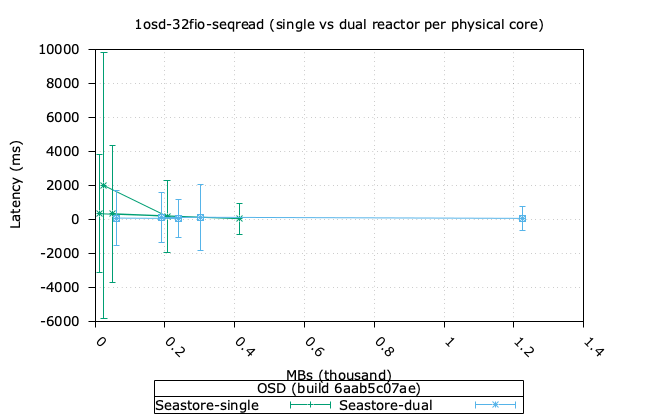
\includegraphics[width=0.9\textwidth]{seastore_1osd_32fio_seqread_iops_vs_lat.png}
  %\caption{Response latency curves, IOPs vs. Latency}
\end{figure}

% utilisation:OSD
% \begin{figure}[h]
%   \centering
%   \begin{minipage}{.5\textwidth}
%   \centering
%     \includegraphics[width=\textwidth]{classic_vs_seastore_1osd_32fio_seqread_iops_vs_lat_osd_cpu.png}
%     %\caption{4k random write}
%      %\label{figure:sea_4k_seqread}
%   \end{minipage}%
%   \begin{minipage}{.5\textwidth}
%   \centering
%     \includegraphics[width=\textwidth]{classic_vs_seastore_1osd_32fio_seqread_iops_vs_lat_osd_mem.png}
%     %\caption{System CPU utilisation}
%     %\label{figure:sea_4k_seqread}
%   \end{minipage}%
% \end{figure}
%
\subsection{Single reactor}

\begin{table}[h!]
\centering
\begin{tabular}[t]{*{11 }{|c|}}
\hline 
iodepth & bw & total\_ios & clat\_ms & clat\_stdev & usr\_cpu & sys\_cpu & OSD\_cpu & OSD\_mem & FIO\_cpu & FIO\_mem\\
\hline
1  & 176.76  & 123918.00  & 11.52  & 623.37  & 0.06  & 0.05  & 0.00  & 0.00  & 19.33  & 20.58 \\
\hline
2  & 11.58  & 7183.00  & 313.32  & 3461.30  & 0.00  & 0.00  & 0.00  & 0.00  & 8.77  & 0.00 \\
\hline
4  & 413.82  & 451651.00  & 19.72  & 901.86  & 0.12  & 0.10  & 0.00  & 0.00  & 64.49  & 34.50 \\
\hline
8  & 49.72  & 42396.00  & 316.17  & 4025.28  & 0.03  & 0.03  & 0.00  & 0.00  & 13.67  & 28.50 \\
\hline
16  & 205.82  & 127744.00  & 158.20  & 2136.51  & 0.06  & 0.05  & 0.00  & 0.00  & 28.51  & 21.00 \\
\hline
24  & 24.80  & 12775.00  & 1971.73  & 7829.85  & 0.01  & 0.01  & 0.00  & 0.00  & 9.13  & 18.00 \\
\hline
32  & 45.89  & 34797.00  & 1413.69  & 8086.52  & 0.02  & 0.02  & 0.00  & 0.00  & 15.40  & 25.50 \\
\hline
40  & 775.16  & 852914.00  & 105.21  & 1883.88  & 0.18  & 0.16  & 0.00  & 0.00  & 110.62  & 36.00 \\
\hline
52  & 1455.32  & 2063347.00  & 72.70  & 1246.43  & 0.32  & 0.30  & 0.00  & 0.00  & 237.54  & 73.50 \\
\hline
64  & 1497.58  & 2109407.00  & 82.75  & 1307.90  & 0.34  & 0.32  & 0.00  & 0.00  & 241.70  & 74.08 \\
\hline

\hline
\end{tabular}
  \caption{Performance Throughput vs Latency vs CPU util: sequential read 64k, single reactor per CPU core.}
  %sea_1osd_28reactor_32fio_bal_osd_rc_1procs_seqread.}
\label{table:iops-lat-cpu-sea_1osd_28reactor_32fio_bal_osd_rc_1procs_seqread}
\end{table}

\subsection{Dual reactor}

\begin{table}[h!]
\centering
\begin{tabular}[t]{*{11 }{|c|}}
\hline 
iodepth & bw & total\_ios & clat\_ms & clat\_stdev & usr\_cpu & sys\_cpu & OSD\_cpu & OSD\_mem & FIO\_cpu & FIO\_mem\\
\hline
1  & 1475.63  & 6917107.00  & 1.38  & 0.75  & 0.47  & 0.39  & 0.00  & 0.00  & 267.87  & 60.00 \\
\hline
2  & 157.79  & 196886.00  & 25.87  & 1288.77  & 0.05  & 0.05  & 0.00  & 0.00  & 48.34  & 42.00 \\
\hline
4  & 1634.39  & 7661467.00  & 5.01  & 3.42  & 0.49  & 0.41  & 0.00  & 0.00  & 249.65  & 43.50 \\
\hline
8  & 432.90  & 407648.00  & 37.77  & 1196.85  & 0.11  & 0.10  & 0.00  & 0.00  & 74.69  & 34.50 \\
\hline
16  & 1827.27  & 8565934.00  & 17.92  & 15.61  & 0.51  & 0.44  & 0.00  & 0.00  & 268.83  & 57.00 \\
\hline
24  & 2160.48  & 10128164.00  & 22.73  & 22.92  & 0.55  & 0.49  & 0.00  & 0.00  & 374.67  & 84.00 \\
\hline
32  & 2186.52  & 10252621.00  & 29.94  & 32.41  & 0.55  & 0.49  & 0.00  & 0.00  & 375.26  & 87.00 \\
\hline
40  & 2310.41  & 10832232.00  & 35.41  & 43.10  & 0.57  & 0.52  & 0.00  & 0.00  & 395.62  & 90.00 \\
\hline
52  & 2370.57  & 11116145.00  & 44.85  & 59.33  & 0.58  & 0.52  & 0.00  & 0.00  & 403.19  & 91.50 \\
\hline
64  & 69.91  & 53785.00  & 1797.92  & 9152.80  & 0.02  & 0.02  & 0.00  & 0.00  & 30.19  & 30.57 \\
\hline

\hline
\end{tabular}
\caption{Performance Throughput vs Latency vs CPU util: sea_1osd_56reactor_32fio_bal_osd_rc_1procs_seqread.}
\label{table:iops-lat-cpu-sea_1osd_56reactor_32fio_bal_osd_rc_1procs_seqread}
\end{table}

%\newpage
\pagebreak

\section{Sequential write 64k}

\begin{figure}[ht]
  \centering
  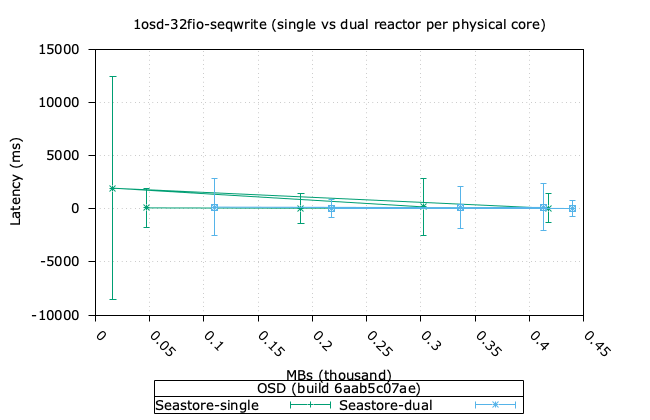
\includegraphics[width=0.9\textwidth]{seastore_1osd_32fio_seqwrite_iops_vs_lat.png}
  %\caption{Response latency curves, IOPs vs. Latency}
\end{figure}

% % utilisation:OSD
% \begin{figure}[h]
%   \centering
%   \begin{minipage}{.5\textwidth}
%   \centering
%     \includegraphics[width=\textwidth]{classic_vs_seastore_1osd_32fio_seqwrite_iops_vs_lat_osd_cpu.png}
%     %\caption{4k random write}
%      %\label{figure:sea_4k_seqwrite}
%   \end{minipage}%
%   \begin{minipage}{.5\textwidth}
%   \centering
%     \includegraphics[width=\textwidth]{classic_vs_seastore_1osd_32fio_seqwrite_iops_vs_lat_osd_mem.png}
%     %\caption{System CPU utilisation}
%     %\label{figure:sea_4k_seqwrite}
%   \end{minipage}%
% \end{figure}
%
\subsection{Single reactor}
../data//osd_1_28reactor_28fio_rc_seastore/sea_1osd_28reactor_32fio_bal_osd_rc_1procs_seqwrite_d/sea_1osd_28reactor_32fio_bal_osd_rc_1procs_seqwrite.tex
\subsection{Dual reactor}

\begin{table}[h!]
\centering
\begin{tabular}[t]{*{11 }{|c|}}
\hline 
iodepth & bw & total\_ios & clat\_ms & clat\_stdev & usr\_cpu & sys\_cpu & OSD\_cpu & OSD\_mem & FIO\_cpu & FIO\_mem\\
\hline
128  & 782.64  & 1771428.00  & 2.27  & 233.97  & 0.68  & 0.24  & 0.00  & 0.00  & 229.11  & 37.94 \\
\hline

\hline
\end{tabular}
\caption{Performance Throughput vs Latency vs CPU util: sea_1osd_56reactor_32fio_bal_osd_rc_1procs_seqwrite.}
\label{table:iops-lat-cpu-sea_1osd_56reactor_32fio_bal_osd_rc_1procs_seqwrite}
\end{table}

%\newpage


